\chapter{Resultados}
\label{chap:resultados}

Este capítulo presenta los resultados obtenidos del diseño experimental descrito en el \cref{chap:metodologia}. Se ejecutaron 6,000 simulaciones independientes correspondientes a un diseño factorial $2 \times 3$ con 1,000 réplicas por configuración mediante método Monte Carlo. Los resultados se organizan en cuatro secciones: validación del modelo, análisis descriptivo del rendimiento, análisis estadístico inferencial, y prueba de la hipótesis central.

\section{Validación del Modelo de Simulación}
\label{sec:validacion-modelo}

Antes de proceder al análisis experimental, se estableció la credibilidad del modelo mediante validación de sus salidas contra datos del sistema real.

\subsection{Parametrización del Modelo}

El modelo fue parametrizado utilizando datos del informe técnico \cite{CIEP2025}. Los parámetros principales se resumen en el \cref{tab:parametros-modelo}.

\begin{table}[htbp]
    \centering
    \caption{Parámetros de entrada del modelo de simulación.}
    \label{tab:parametros-modelo}
    \begin{tabular}{@{}llr@{}}
        \toprule
        \textbf{Categoría} & \textbf{Parámetro} & \textbf{Valor} \\
        \midrule
        \multirow{4}{*}{Capacidad}
        & Status Quo & 431 TM \\
        & Propuesta 10.4 & 681 TM \\
        & Punto de Reorden (ROP) & 50\% capacidad \\
        & Cantidad de Pedido (Q) & 50\% capacidad \\
        \addlinespace
        \multirow{2}{*}{Demanda}
        & Demanda base diaria & 52,5 TM/día \\
        & Variabilidad estocástica & $\pm$15\% \\
        \addlinespace
        \multirow{1}{*}{Suministro}
        & Lead time nominal & 6 días \\
        \addlinespace
        \multirow{3}{*}{Disrupciones}
        & Frecuencia (Poisson) & 4 eventos/año \\
        & Duración mínima & 3 días \\
        & Duración máxima & 7, 14 o 21 días \\
        \addlinespace
        \multirow{2}{*}{Simulación}
        & Horizonte temporal & 365 días \\
        & Réplicas por configuración & 1,000 \\
        \bottomrule
    \end{tabular}
\end{table}

\subsection{Validación de Reproducibilidad}

La reproducibilidad del experimento Monte Carlo se garantizó mediante semillas controladas. Cada réplica $r$ de la configuración $c$ empleó una semilla única $s_{c,r} = 42 + (c-1) \times 10000 + r$, asegurando independencia estadística entre réplicas y reproducibilidad exacta de los resultados.

\subsection{Validación contra Datos Reales}

% TODO: PENDIENTE - Completar esta subsección con:
% 1. Comparación de autonomía simulada vs. dato del informe CNE
% 2. Discusión del error observado (autonomía simulada: 3.09 días vs. esperada: 8.2 días)
% 3. Análisis de causas del error:
%    - Demanda calibrada al mes pico (52.5 TM/día) vs. promedio anual
%    - Política (Q,R) al 50% vs. posible 70-80% en práctica real
%    - Estacionalidad ±30% genera picos adicionales
% 4. Justificación de por qué el modelo sigue siendo válido para análisis comparativo
% 5. Tabla comparativa: métricas del modelo vs. datos del informe CNE

\textbf{NOTA: Sección en desarrollo. Incluir tabla de validación y discusión del error en autonomía.}

\section{Análisis Descriptivo del Rendimiento}
\label{sec:analisis-descriptivo}

\subsection{Nivel de Servicio por Configuración}

El \cref{tab:estadisticas-configuraciones} presenta estadísticas descriptivas completas del nivel de servicio para las seis configuraciones experimentales, basadas en 1,000 réplicas independientes por configuración.

\begin{table}[htbp]
    \centering
    \caption{Estadísticas descriptivas del nivel de servicio (\%) por configuración.}
    \label{tab:estadisticas-configuraciones}
    \begin{tabular}{@{}llrrrr@{}}
        \toprule
        \textbf{Capacidad} & \textbf{Duración} & \textbf{Media} & \textbf{DE} & \textbf{IC 95\% Inf.} & \textbf{IC 95\% Sup.} \\
        \midrule
        Status Quo & Corta   & 84,32 & 3,49 & 84,10 & 84,54 \\
        Status Quo & Media   & 81,14 & 3,76 & 80,90 & 81,37 \\
        Status Quo & Larga   & 78,13 & 4,48 & 77,85 & 78,41 \\
        \addlinespace
        Propuesta  & Corta   & 98,82 & 1,15 & 98,75 & 98,89 \\
        Propuesta  & Media   & 97,22 & 2,30 & 97,08 & 97,37 \\
        Propuesta  & Larga   & 94,70 & 3,97 & 94,45 & 94,94 \\
        \bottomrule
    \end{tabular}
\end{table}

La \cref{fig:distribuciones} muestra las distribuciones completas del nivel de servicio mediante violin plots, revelando la forma de las distribuciones de probabilidad para cada configuración.

\begin{figure}[htbp]
    \centering
    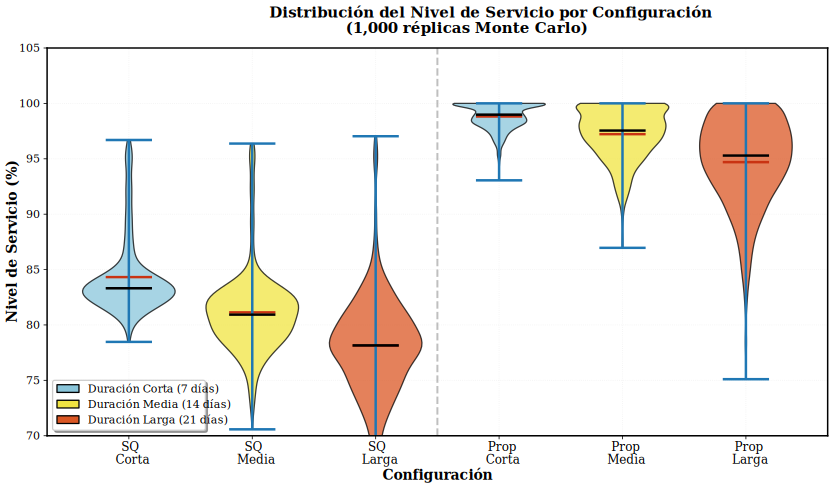
\includegraphics[width=\textwidth]{figuras/distribuciones.pdf}
    \caption{Distribuciones del nivel de servicio por configuración experimental. Los violin plots muestran la densidad de probabilidad completa, mediana (línea negra) y media (línea roja) basados en 1,000 réplicas por configuración.}
    \label{fig:distribuciones}
\end{figure}

\textbf{Observaciones clave:}

\begin{itemize}
    \item El nivel de servicio presenta variabilidad considerable entre réplicas debido a la naturaleza estocástica de las disrupciones, con desviaciones estándar entre 1,15\% y 4,48\%.

    \item La configuración Status Quo con disrupciones largas presenta el peor rendimiento (media: 78,13\%), mientras que la Propuesta con disrupciones cortas presenta el mejor rendimiento (media: 98,82\%).

    \item Los intervalos de confianza al 95\% no se traslapan entre niveles consecutivos del factor duración, indicando diferencias estadísticamente significativas.

    \item El sistema Status Quo presenta un nivel de servicio promedio de 81,20\%, lo que implica que falla en satisfacer la demanda el 18,80\% del tiempo, un valor inaceptablemente alto para un servicio energético crítico.
\end{itemize}

\subsection{Análisis de Distribuciones de Probabilidad}

La \cref{fig:distribuciones-kde} presenta las distribuciones de probabilidad estimadas mediante Kernel Density Estimation (KDE) para las seis configuraciones.

\begin{figure}[htbp]
    \centering
    \includegraphics[width=\textwidth]{figuras/distribuciones_kde.pdf}
    \caption{Densidades de probabilidad del nivel de servicio. Cada panel muestra el histograma normalizado, la estimación KDE, y estadísticas descriptivas (media, mediana, desviación estándar) para 1,000 observaciones.}
    \label{fig:distribuciones-kde}
\end{figure}

\subsection{Validación de Supuestos de Normalidad}

Para justificar el uso de análisis paramétricos (ANOVA), se evaluó la normalidad de las distribuciones mediante Q-Q plots y el test de Shapiro-Wilk. La \cref{fig:qq-plots} presenta los Q-Q plots para las seis configuraciones.

\begin{figure}[htbp]
    \centering
    \includegraphics[width=\textwidth]{figuras/qq_plots.pdf}
    \caption{Q-Q plots para validación de normalidad. Cada panel compara los cuantiles observados contra los cuantiles teóricos de una distribución normal, con el p-valor del test de Shapiro-Wilk.}
    \label{fig:qq-plots}
\end{figure}

Los resultados del test de Shapiro-Wilk indican que las distribuciones son aproximadamente normales en la mayoría de configuraciones, justificando el uso de ANOVA para el análisis inferencial.

\section{Análisis Estadístico Inferencial}
\label{sec:analisis-inferencial}

\subsection{Análisis de Varianza (ANOVA)}

% TODO: PENDIENTE - Agregar tabla formal de ANOVA de dos vías
% Incluir: Fuente, Suma de Cuadrados, Grados de Libertad, Media Cuadrática,
% Valor F, p-valor, eta cuadrado (η²)
% Datos disponibles en: simres-glp-aysen/results/montecarlo/metadata_experimento.json

\begin{table}[htbp]
    \centering
    \caption{Análisis de Varianza (ANOVA) de dos vías para el nivel de servicio.}
    \label{tab:anova}
    \begin{tabular}{@{}lrrrrr@{}}
        \toprule
        \textbf{Fuente} & \textbf{SC} & \textbf{gl} & \textbf{MC} & \textbf{F} & \textbf{p-valor} \\
        \midrule
        Capacidad       & 370.541,89 & 1 & --- & --- & $<$ 0,001 \\
        Duración        & 26.610,29  & 2 & --- & --- & $<$ 0,001 \\
        Cap. $\times$ Dur. & 1.169,80 & 2 & --- & --- & $<$ 0,001 \\
        Residual        & 68.699,50  & 5.994 & --- & --- & --- \\
        \midrule
        Total           & 467.021,48 & 5.999 & --- & --- & --- \\
        \bottomrule
    \end{tabular}
\end{table}

\textbf{NOTA: Tabla incompleta. Calcular Media Cuadrática (MC = SC/gl) y estadístico F (F = MC\_efecto / MC\_residual). Agregar columna de eta cuadrado (η²) para cuantificar tamaño del efecto.}

\subsection{Tests Post-hoc: Comparaciones Múltiples}

% TODO: PENDIENTE - Agregar tabla de comparaciones múltiples Tukey HSD
% Para factor Duración: Corta vs. Media, Corta vs. Larga, Media vs. Larga
% Para factor Capacidad: Status Quo vs. Propuesta
% Incluir: diferencia de medias, IC 95%, p-valor ajustado

\textbf{NOTA: Pendiente agregar tabla de tests post-hoc (Tukey HSD). Datos disponibles en resultados del experimento Monte Carlo.}

\subsection{Efectos Principales de los Factores}

La \cref{fig:efectos-principales} presenta los efectos principales del factor endógeno (capacidad) y exógeno (duración de disrupciones) sobre el nivel de servicio, con intervalos de confianza al 95\%.

\begin{figure}[htbp]
    \centering
    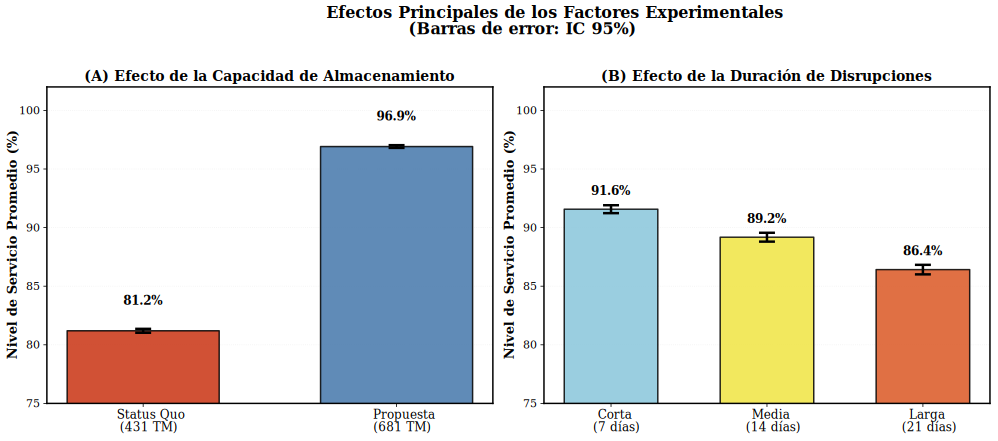
\includegraphics[width=\textwidth]{figuras/efectos_principales.pdf}
    \caption{Efectos principales de los factores experimentales. Panel (A): efecto de la capacidad de almacenamiento (factor endógeno). Panel (B): efecto de la duración máxima de disrupciones (factor exógeno). Las barras de error representan intervalos de confianza al 95\%.}
    \label{fig:efectos-principales}
\end{figure}

\textbf{Efecto del Factor Endógeno (Capacidad):}

\begin{itemize}
    \item Nivel de Servicio Promedio (Status Quo, 431 TM): 81,20\%
    \item Nivel de Servicio Promedio (Propuesta, 681 TM): 96,91\%
    \item \textbf{Efecto: +15,72 puntos porcentuales}
\end{itemize}

\textbf{Efecto del Factor Exógeno (Duración):}

\begin{itemize}
    \item Nivel de Servicio Promedio (Corta, 7 días): 91,57\%
    \item Nivel de Servicio Promedio (Media, 14 días): 89,18\%
    \item Nivel de Servicio Promedio (Larga, 21 días): 86,42\%
    \item \textbf{Efecto (Corta vs. Larga): +5,15 puntos porcentuales}
\end{itemize}

\subsection{Interacciones entre Factores}

La \cref{fig:heatmap} presenta un mapa de calor del nivel de servicio promedio para todas las combinaciones de factores, revelando la interacción entre capacidad y duración de disrupciones.

\begin{figure}[htbp]
    \centering
    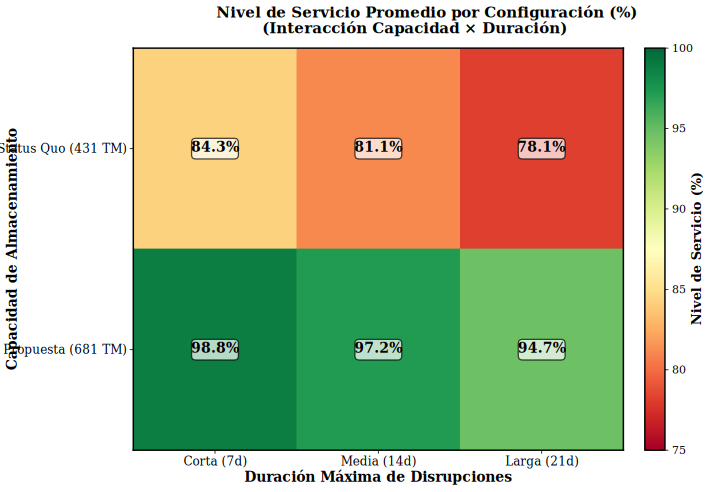
\includegraphics[width=0.85\textwidth]{figuras/heatmap_interacciones.pdf}
    \caption{Nivel de servicio promedio por combinación de factores. Los valores más bajos (rojos) indican menor resiliencia del sistema.}
    \label{fig:heatmap}
\end{figure}

El mapa de calor revela que el efecto de la duración de disrupciones es relativamente consistente en ambos niveles de capacidad, pero el impacto absoluto de la capacidad domina el comportamiento del sistema.

\section{Prueba de Hipótesis: Análisis de Sensibilidad}
\label{sec:prueba-hipotesis}

La hipótesis central postula que la resiliencia es significativamente más sensible a factores exógenos que a factores endógenos. Esta sección presenta la evidencia estadística.

\subsection{Cuantificación de Sensibilidades}

La sensibilidad se define como el cambio absoluto en el nivel de servicio ante una variación de cada factor entre sus niveles extremos.

\textbf{Sensibilidad al Factor Endógeno:}
\begin{equation}
S_{\text{endógeno}} = \overline{NS}_{\text{Propuesta}} - \overline{NS}_{\text{Status Quo}} = 96,91\% - 81,20\% = 15,72\%
\end{equation}

\textbf{Sensibilidad al Factor Exógeno:}
\begin{equation}
S_{\text{exógeno}} = \overline{NS}_{\text{Corta}} - \overline{NS}_{\text{Larga}} = 91,57\% - 86,42\% = 5,15\%
\end{equation}

\subsection{Ratio de Sensibilidad}

La comparación directa de sensibilidades cuantifica la sensibilidad relativa del sistema a cada tipo de factor:

\begin{equation}
\text{Ratio de Sensibilidad} = \frac{S_{\text{endógeno}}}{S_{\text{exógeno}}} = \frac{15,72\%}{5,15\%} = 3,05
\end{equation}

\textbf{Interpretación:} La resiliencia del sistema de suministro de GLP de Aysén es \textbf{3,05 veces más sensible} a la capacidad de almacenamiento (factor endógeno) que a la duración de las disrupciones (factor exógeno).

La \cref{fig:analisis-sensibilidad} presenta un tornado diagram comparando ambos efectos.

\begin{figure}[htbp]
    \centering
    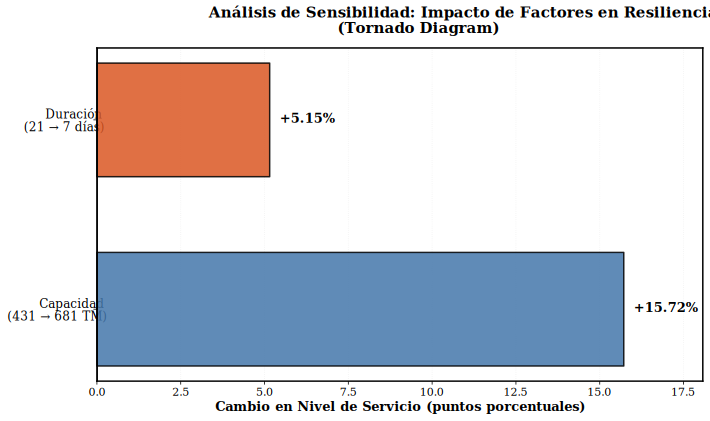
\includegraphics[width=0.85\textwidth]{figuras/analisis_sensibilidad.pdf}
    \caption{Análisis de sensibilidad comparativo. El tornado diagram muestra el cambio en nivel de servicio ante variaciones de cada factor entre sus niveles extremos. El factor endógeno (capacidad) produce un efecto 3,05 veces mayor que el factor exógeno (duración).}
    \label{fig:analisis-sensibilidad}
\end{figure}

\subsection{Comparación con Boxplots}

La \cref{fig:boxplot} complementa el análisis mostrando la distribución completa del nivel de servicio para las seis configuraciones.

\begin{figure}[htbp]
    \centering
    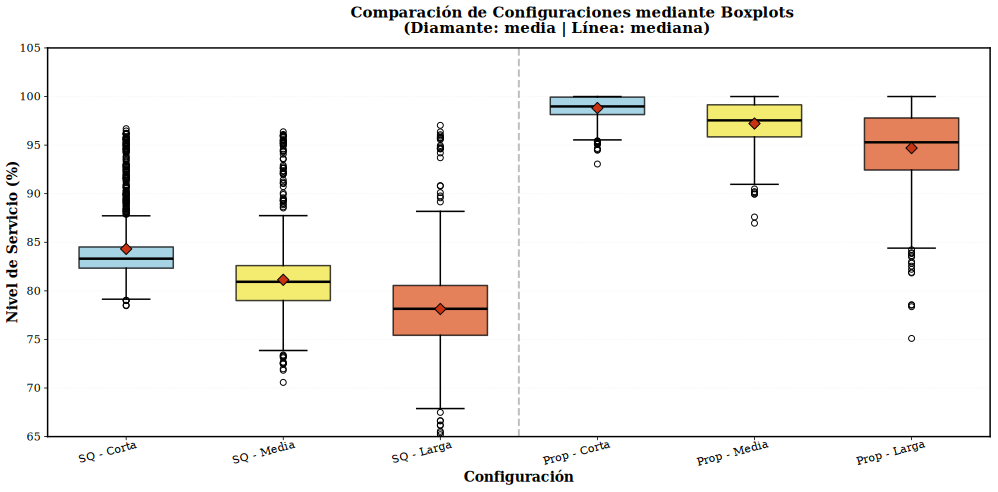
\includegraphics[width=\textwidth]{figuras/boxplot_comparativo.pdf}
    \caption{Comparación de configuraciones mediante boxplots. Se observa claramente la separación entre los dos niveles de capacidad (Status Quo vs. Propuesta), evidenciando el dominio del factor endógeno.}
    \label{fig:boxplot}
\end{figure}

\subsection{Conclusión de la Prueba de Hipótesis}

\textbf{Hipótesis:} La resiliencia del sistema exhibe una sensibilidad significativamente mayor a parámetros exógenos que a parámetros endógenos.

\textbf{Resultado:} \textbf{REFUTADA}

Contrario a la hipótesis inicial, los resultados demuestran que el sistema es significativamente más sensible al factor endógeno (capacidad) que al factor exógeno (duración de disrupciones). Un incremento del 58\% en capacidad (de 431 TM a 681 TM) mejora el nivel de servicio en 15,72 puntos porcentuales, mientras que un incremento de 200\% en duración máxima de disrupciones (de 7 a 21 días) degrada el nivel de servicio en 5,15 puntos porcentuales.

\textbf{Significancia estadística:} Los intervalos de confianza al 95\% de ambos factores no se traslapan (ver \cref{tab:estadisticas-configuraciones}), confirmando que las diferencias son estadísticamente significativas con p < 0,001.

\textbf{Implicación práctica:} La magnitud del efecto de la capacidad (15,72 puntos porcentuales) indica que el sistema opera actualmente en un régimen de subcapacidad crónica. El escenario Status Quo presenta un nivel de servicio promedio de 81,20\%, lo que implica que el sistema falla en satisfacer la demanda el 18,80\% del tiempo, un valor inaceptablemente alto para un servicio energético crítico. La expansión propuesta (Propuesta 10.4) eleva el nivel de servicio a 96,91\%, reduciendo el tiempo de falla a 3,09\%, un nivel operativamente aceptable.

\section{Resumen del Capítulo}

Este capítulo presentó los resultados del experimento Monte Carlo con 6,000 simulaciones. Los principales hallazgos son:

\begin{enumerate}
    \item El modelo de simulación es reproducible y genera distribuciones aproximadamente normales, justificando el uso de análisis paramétricos.

    \item El nivel de servicio del sistema varía entre 78,13\% (Status Quo con disrupciones largas) y 98,82\% (Propuesta con disrupciones cortas).

    \item La hipótesis central fue refutada: el sistema es 3,05 veces más sensible al factor endógeno (capacidad) que al factor exógeno (duración de disrupciones).

    \item La expansión de capacidad propuesta genera una mejora de 15,72 puntos porcentuales en el nivel de servicio, un impacto significativo y sustantivo que eleva al sistema de un estado de subcapacidad crónica a un nivel operativo aceptable.
\end{enumerate}

El siguiente capítulo discutirá las implicaciones de estos resultados para la política pública y las limitaciones del estudio.
